%% derived from https://tex.stackexchange.com/questions/357538/graph-of-a-parabola-on-pgfplots
%% Thanks to Stefan Pinnow
%%     https://tex.stackexchange.com/users/95441/stefan-pinnow

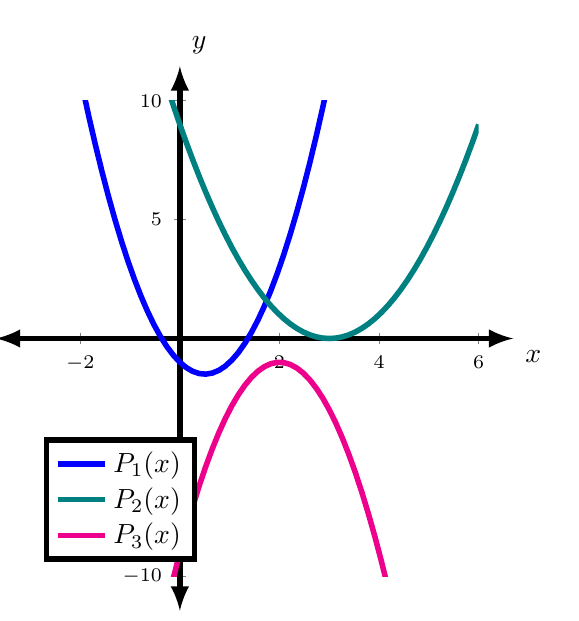
\begin{tikzpicture}
  \begin{axis}[
      legend pos=south west,
      width=.6\textwidth,
      height=3in,
      axis lines=middle,
      xmin=-3,
      xmax=6,
      ymin=-10,
      ymax=10,
      scaled ticks=false,
      line width=2pt,
      ticklabel style={font=\scriptsize},
      xlabel=$x$,
      ylabel=$y$,
      samples=70,
      domain=-3:6,
      axis line style={
        latex-latex,
        shorten >=-12.5pt,
        shorten <=-12.5pt,
      },
      xlabel style={at={(ticklabel* cs:1)}, xshift=12.5pt, anchor=north west},
      ylabel style={at={(ticklabel* cs:1)}, yshift=12.5pt, anchor=south west},
    ]
    
    \addplot[color=blue] {2*x^2 - 2*x - 1}; % 2 roots
    \addlegendentry{\(P_1(x)\)}
    \addplot[color=teal] {x^2 - 6*x + 9}; % 1 root
    \addlegendentry{\(P_2(x)\)}
    \addplot[color=magenta] {-2*x^2 + 8*x - 9}; % 0 roots
    \addlegendentry{\(P_3(x)\)}
  \end{axis}
\end{tikzpicture}
%
